\chapter{Desenvolvimento}
\label{c.desenvolvimento}

\section{Utilizando Métodos {\em LossLess}}
\label{s.losslessdev}

Para o método sem perda escolhido foi a Codificação de Huffman, por ser uma técnica simples e fácil de aplicar. A técnica, como descrita no Capítulo 2, se baseia em remover a redundância de bits ao analisar diferentes características ou especificações.

\subsection{Codificação de Huffman}
\label{ss.huffmandev}

O primeiro passo nessa técnica é de reduzir a imagem original em um histograma ordenado, onde a probabilidade de ocorrência de um certo valor de intensidade de um pixel é igual a \[ PP = NP / T \] onde {\em PP} é a probabilidade de ocorrência, {\em NP} é o número de pixels de mesma intensidade e {\em T} o número total de pixels contidos na imagem original.

Histograma é a representação gráfica em colunas ou em barras de um conjunto de dados previamente tabulado e dividido em classes uniformes ou não uniformes.

Dada a seguinte imagem:

\begin{figure}[h]
\caption{\small Imagem 8x8 pixels}
\centering

\includegraphics[scale=0.50]{figs/Input-Image-1.png}
\label{f.imagecompressionbasics}
\end{figure}

Ao se fazer seu histograma, temos:

\begin{table}[]
    \begin{center}
        \caption{\small Valores de intensidade de pixels}
        \label{t.imagecompressionbasics}
        \begin{tabular}{llrlllll}
            128 & 75  & 72  & 105 & 149 & 169 & 127 & 100 \\
            122 & 84  & 83  & 84  & 146 & 138 & 142 & 139 \\
            118 & 98  & 89  & 94  & 136 & 96  & 143 & 188 \\
            122 & 106 & 79  & 115 & 148 & 102 & 127 & 167 \\
            127 & 115 & 106 & 94  & 115 & 124 & 103 & 155 \\
            125 & 115 & 130 & 140 & 170 & 174 & 115 & 136 \\
            127 & 110 & 122 & 163 & 175 & 140 & 119 & 87  \\
            146 & 114 & 127 & 140 & 131 & 142 & 153 & 93
        \end{tabular}
    \end{center}
\end{table}

A imagem contém 46 valores de intensidade distintos, portanto terá 46 símbolos únicos no dicionário de Huffman.

O método de Huffman pode ser separado da seguinte forma:

\begin{alineas}
    \item Construir a Árvore de Huffman
    \item Voltar todo o processo até que chegue ao nó inicial, atribuindo 0 ou 1 para cada nó intermediário, até que chegue ao nó da base.
\end{alineas}

\subsubsection{Construir a Árvore de Huffman}
\label{sss.huffmantree}

A figura \ref{f.imagebeezu} foi utilizada para testes durante o desenvolvimento.

\begin{figure}[h]
\caption{\small beezu.jpg, dimensão 1280x1280, 240KB}
\centering
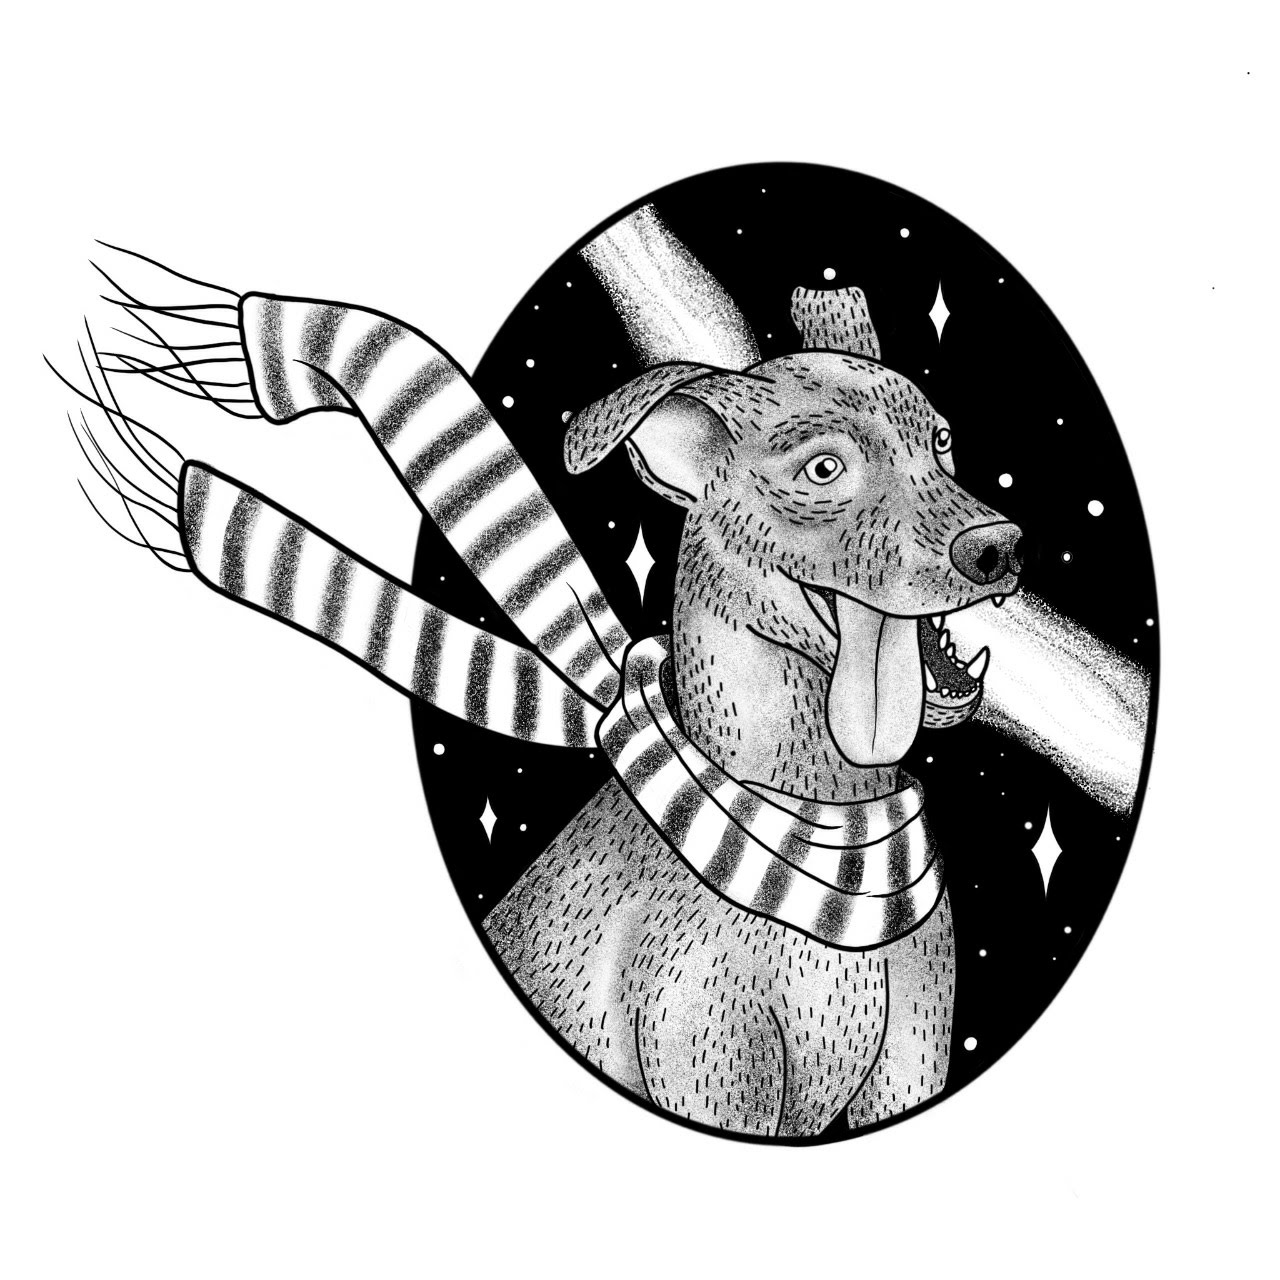
\includegraphics[scale=0.25]{figs/beezu.jpg}
\label{f.imagebeezu}
\end{figure}

Para isso, precisamos primeiramente transformar a cadeia de caracteres da imagem em um vetor de caracteres. Tendo cada caracter num vetor, é feita uma contagem da frequência de cada caracter.

A partir disso é possível construir uma Árvore de Huffman. Isso é feito ao percorrer o {\em array} de frequências, inserindo cada caracter como um nó na Árvore de Huffman partindo pelos dois símbolos de menor frequência, que então são somados em símbolos auxiliares, sendo estes símbolos realocados no conjunto de símbolos. Tendo contruído a Árvore, percorremos ela, atribuindo valores binários para cada aresta.

\begin{figure}[h]
\caption{\small Representação da Árvore de Huffman da Figura 5}
\centering
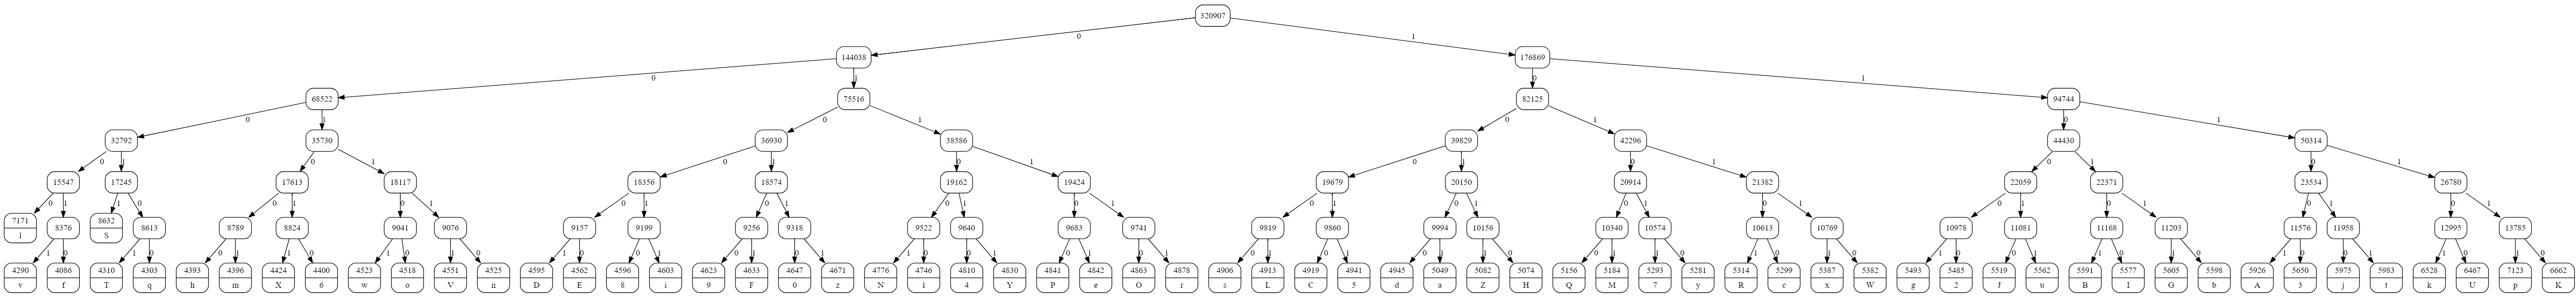
\includegraphics[scale=0.08]{figs/beezu_huffman.PNG}
\label{f.imagebeezutree}
\end{figure}

\subsubsection{Reconstruir a Imagem Utilizando a Árvore de Huffman}
\label{sss.huffmantreebacktrack}

Começando do nó inicial, atribuimos a 0 para a esquerda e 1 para os nós da direita. Como estamos adicionando os nós recém formados ao {\em array} de frequência

\subsubsection{Resultados e Comparações}
\label{sss.results}
%
Pelos testes realizados, já foi possível notar uma diferença no tamanho da cadeia de caracteres gerada pela imagem. A imagem original, sua cadeia de caracteres possui um tamanho de 328864, enquanto que sua versão otimizada 197636.
% \begin{figure}[h]
% \caption{\small Fonte: Original - 240KB}
% \centering
% 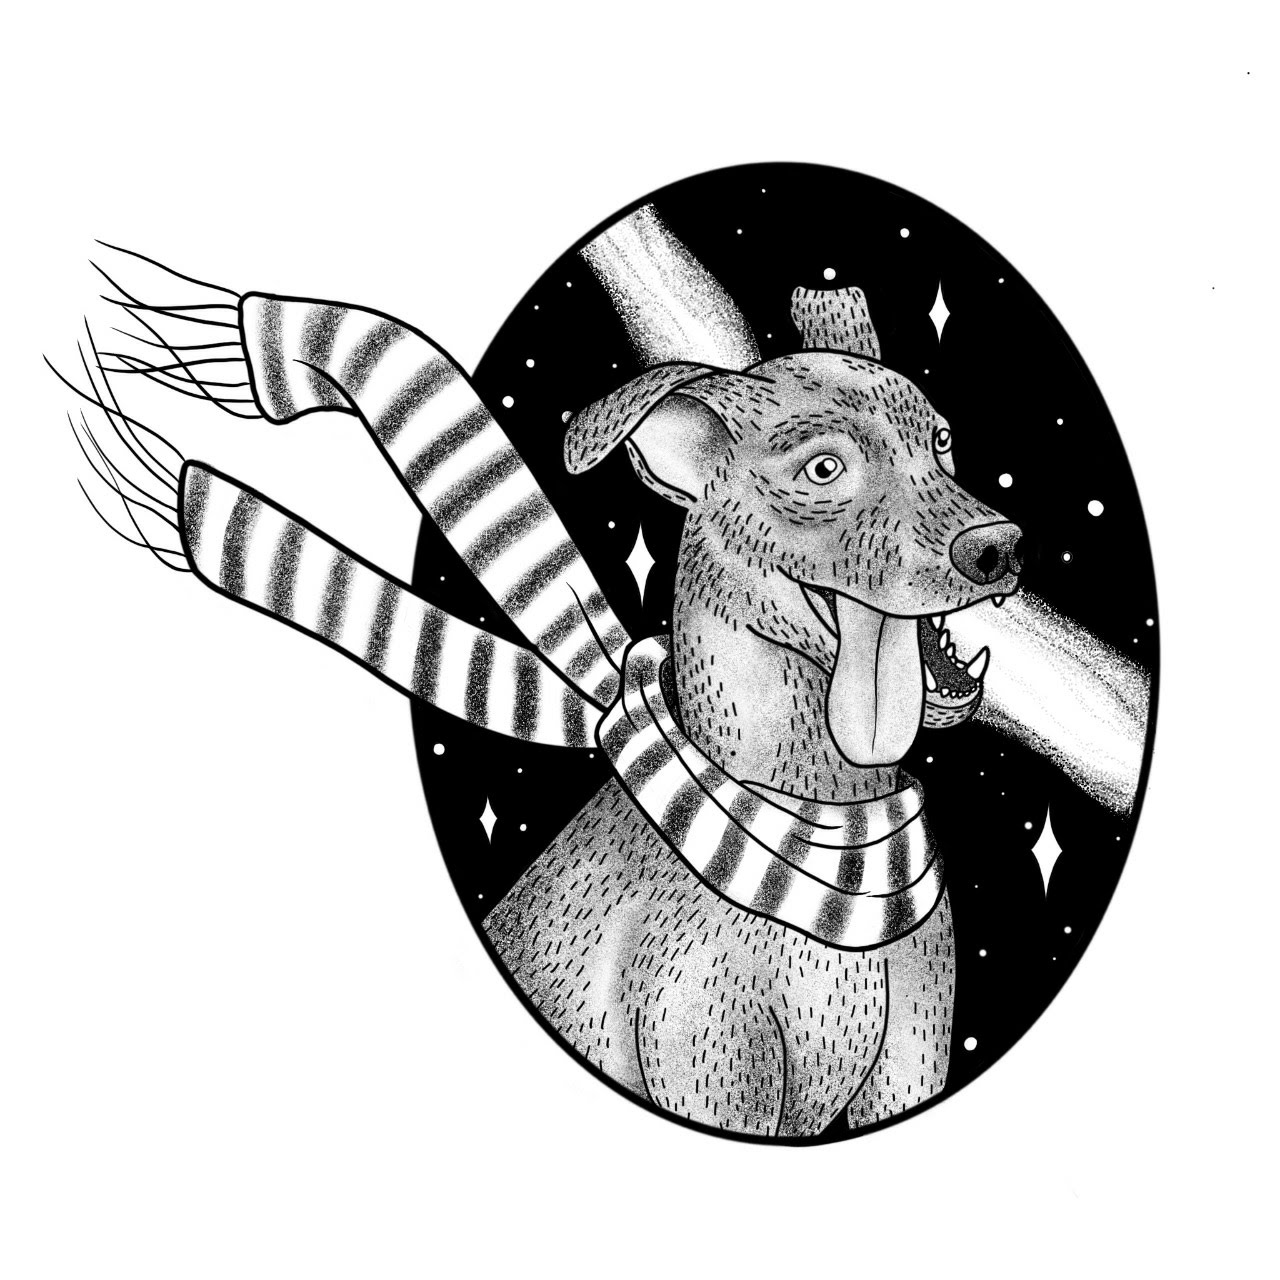
\includegraphics[scale=0.25]{figs/beezu.jpg}
% \label{f.imagebeezuo}
% \end{figure}
%
% \begin{figure}[h]
% \caption{\small Fonte: Testes - 213KB}
% \centering
% 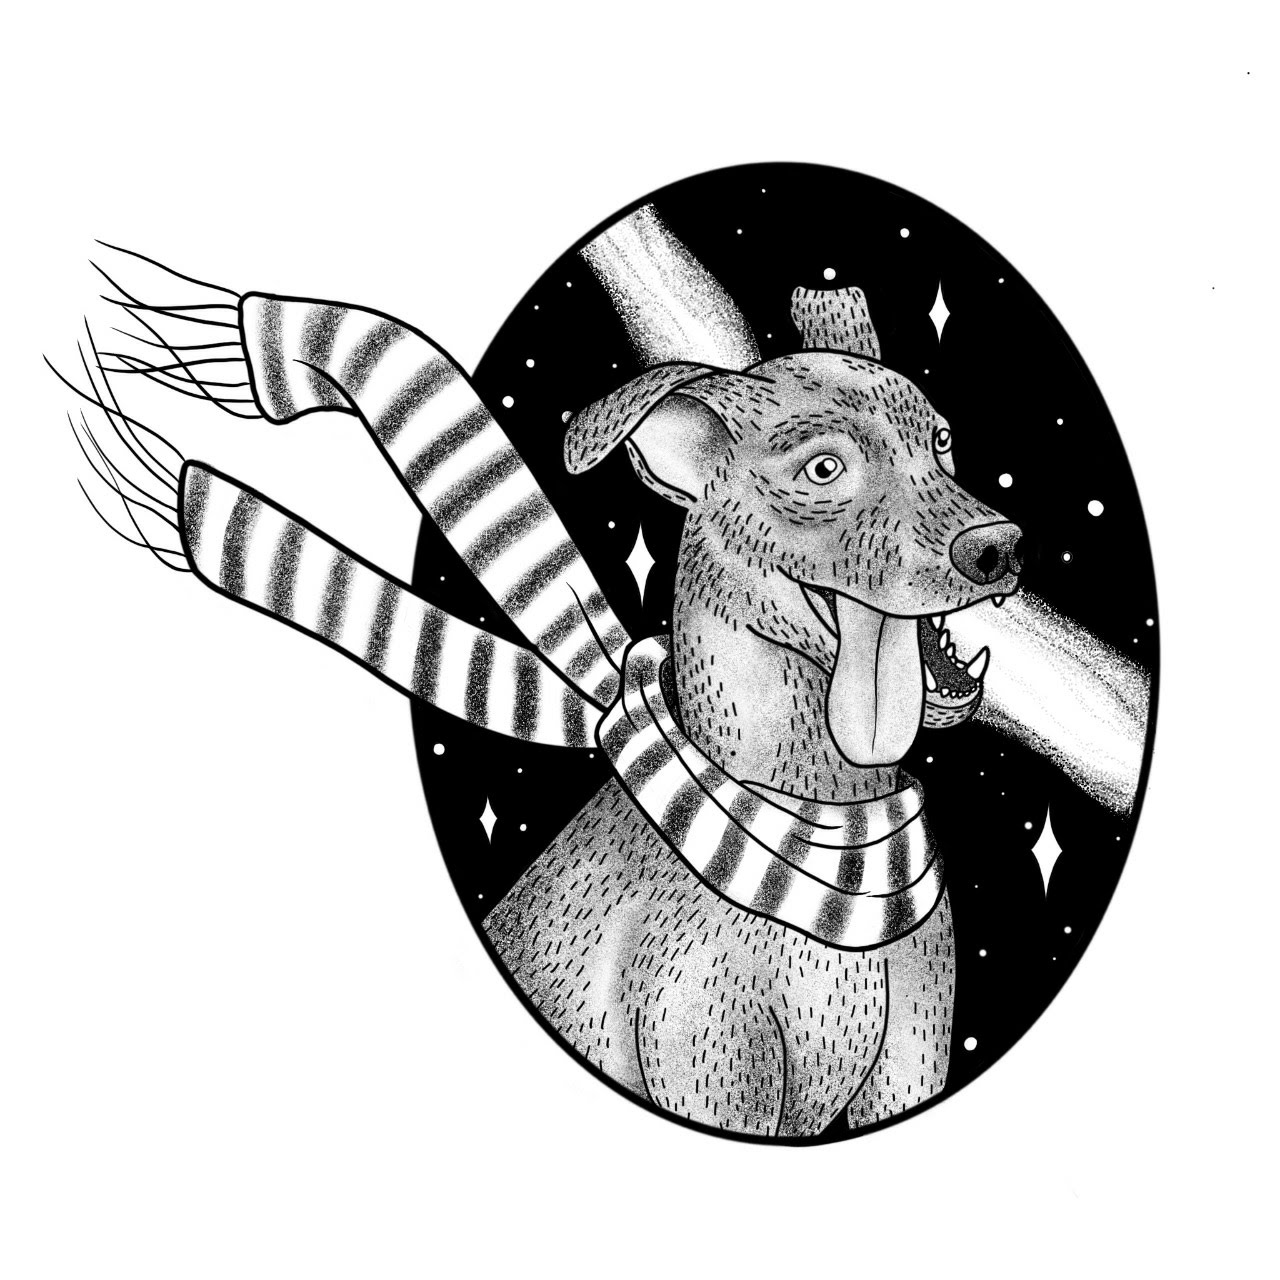
\includegraphics[scale=0.25]{figs/beezu.jpg}
% \label{f.imagebeezur}
% \end{figure}
%
% \begin{figure}[h]
% \caption{\small Fonte: TinyPNG - 141KB}
% \centering
% 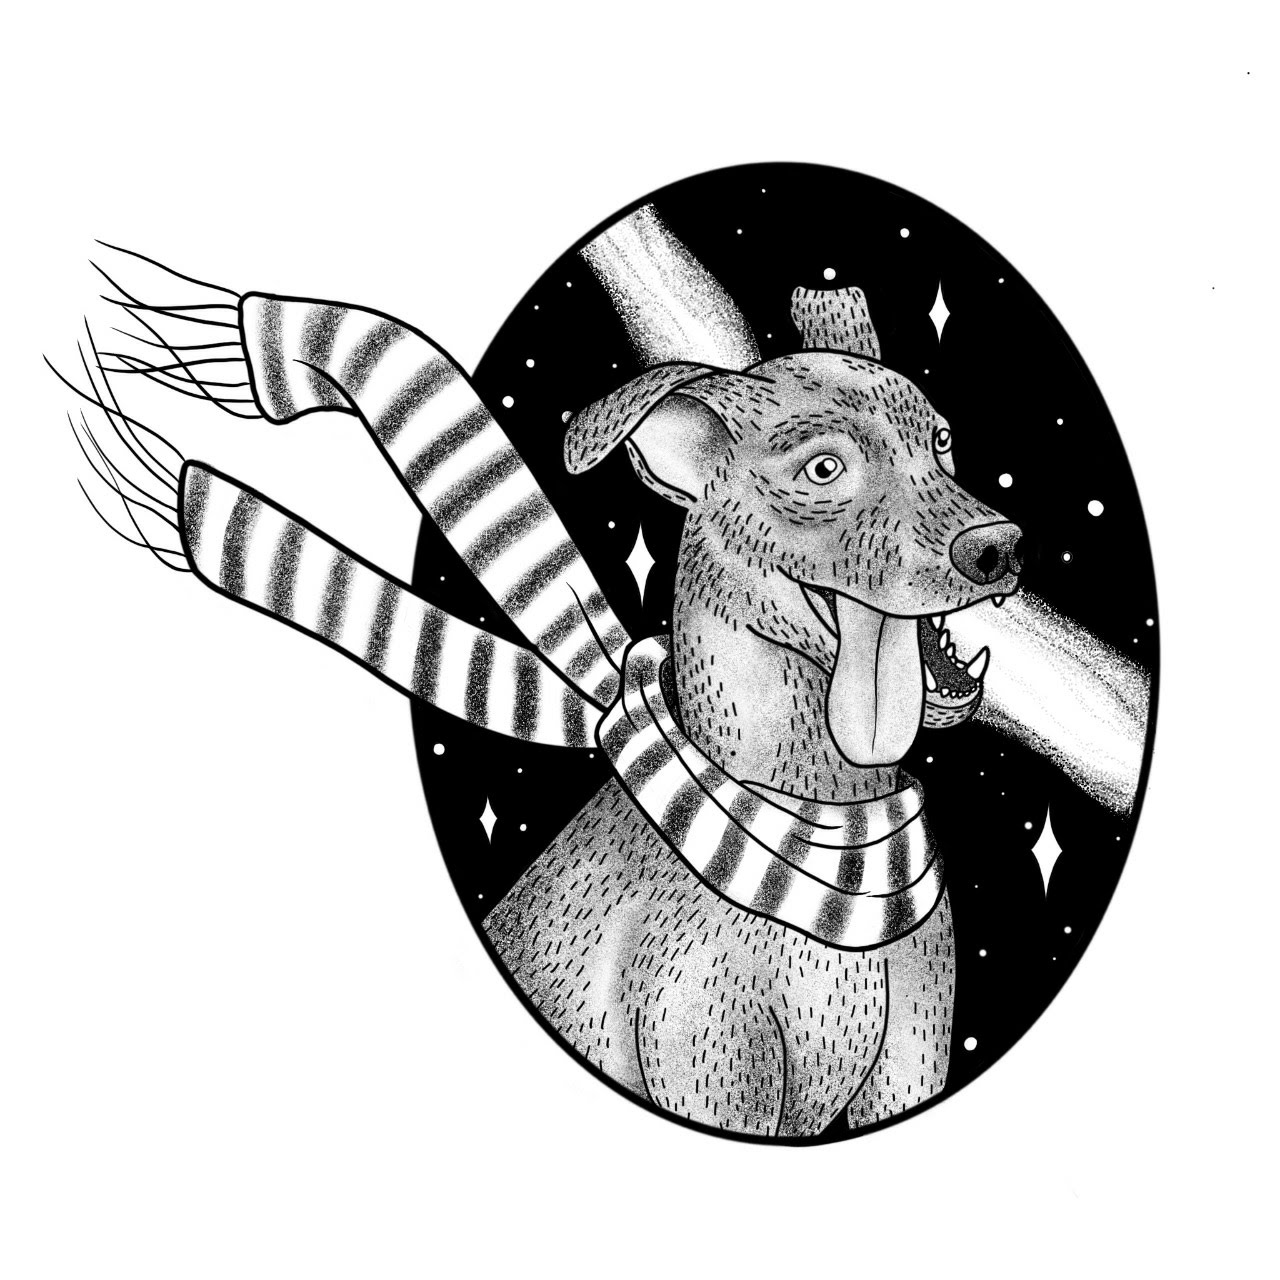
\includegraphics[scale=0.25]{figs/beezu.jpg}
% \label{f.imagebeezut}
% \end{figure}
